\documentclass{article}
\usepackage[utf8]{inputenc}
\usepackage{graphicx}
\usepackage{geometry}
\usepackage{listings}
\usepackage{xcolor}

\usepackage{listings}
\usepackage{color}

\definecolor{mygreen}{rgb}{0,0.6,0}
\definecolor{mygray}{rgb}{0.5,0.5,0.5}

\lstset{ 
  backgroundcolor=\color{white},   % choose the background color; you must add \usepackage{color} or \usepackage{xcolor}; should come as last argument
  basicstyle=\footnotesize,        % the size of the fonts that are used for the code
  breakatwhitespace=false,         % sets if automatic breaks should only happen at whitespace
  breaklines=true,                 % sets automatic line breaking
  captionpos=b,                    % sets the caption-position to bottom
  commentstyle=\color{mygreen},    % comment style
  deletekeywords={...},            % if you want to delete keywords from the given language
  escapeinside={\%*}{*)},          % if you want to add LaTeX within your code
  extendedchars=true,              % lets you use non-ASCII characters; for 8-bits encodings only, does not work with UTF-8
  firstnumber=1,                % start line enumeration with line 1000
  frame=single,	                   % adds a frame around the code
  keepspaces=true,                 % keeps spaces in text, useful for keeping indentation of code (possibly needs columns=flexible)
  keywordstyle=\color{orange},       % keyword style
  language=Python,                 % the language of the code
  morekeywords={*,...},            % if you want to add more keywords to the set
  numbers=left,                    % where to put the line-numbers; possible values are (none, left, right)
  numbersep=5pt,                   % how far the line-numbers are from the code
  numberstyle=\tiny\color{mygray}, % the style that is used for the line-numbers
  rulecolor=\color{black},         % if not set, the frame-color may be changed on line-breaks within not-black text (e.g. comments (green here))
  showspaces=false,                % show spaces everywhere adding particular underscores; it overrides 'showstringspaces'
  showstringspaces=false,          % underline spaces within strings only
  showtabs=false,                  % show tabs within strings adding particular underscores
  stepnumber=2,                    % the step between two line-numbers. If it's 1, each line will be numbered
  stringstyle=\color{pink},     % string literal style
  tabsize=2,	                   % sets default tabsize to 2 spaces
  title=\lstname                   % show the filename of files included with \lstinputlisting; also try caption instead of title
}

\geometry{margin = .7in}
\graphicspath{images}

\title{Assignment 3 CPL}
\author{Harry Haisty}
\date{March 2019}

\begin{document}

\begin{titlepage}
   \begin{center}
       \vspace*{4cm}
 
       \textbf{Assignment 3: Chapter 5 \& 6 -- Names, Bindings, and Data Types}
 
       \vspace{0.5cm}
        CS 4308 -- Concepts of Programming Languages, Professor Sharon Perry

       \vspace{.5cm}
 
       \textbf{Harry Haisty}
       \vfill
 
       \vspace{0.8cm}
 
   \end{center}
\end{titlepage}

\section*{Input Values Used}
The input values I used for this assignment were typeless. There were only three input values used, one for \textsc{student name}, one for \textsc{student number}, and one for \textsc{number of courses}. These values were not hard-coded, they were accepted as user input and then passed to the \textsc{Student} object. 
\newline \newline
Once the \textsc{Student} object was created, the method for displaying the information was called. Since the object already had been passed the variables, all I needed to do was to call \textsc{self.variable}. Since the attributes already existed in the scope, I wrote a formatted string that included prompts and variables in a method I called \textsc{display\_info}, and called that method from \textsc{main}. 
\newline \newline
The final requisite from this program was to prompt the user to change an attribute of the input. For this, I set up a list of variables, and parsed through them randomly. When the choice was made by the machine, it prompted the user to change the corresponding aspect of the student's information. It accepted the user input, and then assigned that new value to the \textsc{Student} object. 

\section*{Platform Used}
The platform I used was PyCharm on Windows, using the on-board output window. 

\section*{Screenshot of Output}
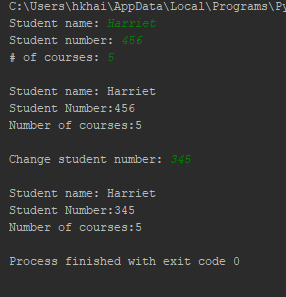
\includegraphics[scale=1]{assignment3}

\newpage

\section*{The Source Code}
\begin{lstlisting}
import random

class Student:
    #adds constructor for Student object
    def __init__(self, name, number, courses):
        self.name = name
        self.number = number
        self.courses = courses

    #creates method to display Student object assigned attributes
    def display_info(self):
        #string formatted to include styling prompts and variable values
        print(f'\nStudent name: {self.name}\nStudent Number:{self.number}\nNumber of courses:{self.courses}')

    #creates method to prompt user to change an attribute in the defined code
    def change_info(self):
        #creates list of variable names to choose
        foo = [self.name, self.number, self.courses]
        #selects random attribute
        choice = random.choice(foo)

        #in case random choice happens to be name attribute
        if choice == self.name:
            #this prompts user to change name and assigns new value
            self.name = input('\nChange student name: ')
            #prints string with new info
            print(f'\nStudent name: {self.name}\nStudent Number:{self.number}\nNumber of courses:{self.courses}')

        #in case random choice happens to be number attribute
        elif choice == self.number:
            #prompts user to change number and assigns new value
            self.number = input('\nChange student number: ')
            #prints string with new info
            print(f'\nStudent name: {self.name}\nStudent Number:{self.number}\nNumber of courses:{self.courses}')

        #in case random choice happens to be course attribute
        else:
            #prompts user to change course number and assigned new value
            self.courses = input('\nChange student courses: ')
            #prints string with new info
            print(f'\nStudent name: {self.name}\nStudent Number:{self.number}\nNumber of courses:{self.courses}')

#main method definition
if __name__ == '__main__':
    #accepts user input for student name
    student_name = input("Student name: ")
    #acepts user input for student number
    student_number = input("Student number: ")
    #accepts user input for student course values
    num_of_courses = input("# of courses: ")

    #creates student object
    stu_1 = Student(student_name, student_number, num_of_courses)
    #calls method to display student info
    stu_1.display_info()
    #calls method to change student info and display
    stu_1.change_info()
\end{lstlisting}



\end{document}
